
\subsection{Selección de un framework de aspectos}  
		Un primer paso para la implementación de la herramienta fue la selección de una
		tecnología que permitiera desarrollar utilizando AOP.
		Con ese objetivo, se evaluaron dos frameworks: Javassist
		\cite{chiba00loadtime} y AspectJ \cite{KiczalesHHKPG01}.
	
	\medskip 
	Encontramos que AspectJ es una herramienta de más alto nivel, que extiende
	el lenguaje Java agregando construcciones específicas para AOP.
	Sin embargo, AspectJ requiere que el programador que use nuestro framework
	utilice un compilador específico, provisto por AspectJ. 
	Consideramos que esta característica es negativa, por condicionar el
	entorno de trabajo de los usuarios de nuestra herramienta.
	
	Javassist, por su lado, aplica los aspectos al momento de
	la carga de las clases, sólo requiere que utilicemos un \emph{ClassLoader}
	específico, resultando menos invasivo para los programadores de aplicaciones
	basadas en nuestra herramienta.
	Como aspecto negativo, notamos que es un framework de muy bajo nivel que
	carece de las abstracciones necesarias para modelar con aspectos y en cambio
	obliga a pensar a nivel de edición de expresiones en el bytecode de una clase
	compilada.
	
	Elegimos Javassist porque priorizamos minimizar el impacto hacia los usuarios
	de nuestra herramienta.
	Para minimizar los problemas asociados a utilizar un framework de tan bajo
	nivel, desarrollamos una herramienta que simplifica su uso, agregando algunas
	abstracciones útiles. Esta herramienta se describe en la sección siguiente.

\subsection{Desarrollo de Aspect for Pure Objects}
	El framework Javassist permite modificar directamente el \emph{bytecode} de
	una clase en el momento de cargarla.
	Por ser de tan bajo nivel es uno de los frameworks de aspectos más poderosos,
	pero, por el mismo motivo, obliga a escribir código muy poco entendible.
	Por eso se desarrolló una herramienta llamada \emph{Aspect for Pure Objects} (APO), 
	que permite definir aspectos utilizando conceptos de más alto nivel y
	aplicárselo a un grupo de objetos. 
	
	La Figura \ref{aopImage} muestra esquemáticamente el diseño de la herramienta.
	Una instancia de \code{AdviceWeaver} se ocupa de aplicar los cambios sobre las
	clases.
	Cada uno de los cambios que debe realizar el \code{AdviceWeaver} está
	modelado por un \code{Advice}, que consiste de un \code{PointCut} y un conjunto de 
	\code{Interceptor}s.
	
	El \code{PointCut} tiene la responsabilidad de determinar el conjunto de
	clases sobre el que aplica el advice. Se provee algunas implementaciones básicas
	de point cuts, por ejemplo, \code{ClassPointCut}, \code{FieldPointCut}, 
	\code{MethodPointCut}, entre otros. Cada uno de estos point cuts tienen un conjunto de funciones
	de filtro, definidas por el usuario programador que use la herramienta. 

	Los \code{Interceptor}s tienen la responsabilidad de realizar las modificaciones sobre 
	los join points de las clases seleccionadas por el point cut. 
 	Cada \code{Interceptor} interepta una acción específica del código, por ejemplo
 	llamadas a métodos, acceso a los atributos, ect. La herramienta provee algunas implementaciones de interceptors,
 	por ejemplo, \code{FieldInterceptor}, \code{MethodInterceptor}, ect. 
 	Cada \code{Interceptor} tiene un conjunto de \code{Behavior}s.
 	Los \code{Behavior} modelan cada modificación a realizar sobre los join points. 
 	Estas modificaciones son modeladas como funciones por el programador.
 	Existen varios tipos de behavior, siguiendo la teoria de AOP: 
 	\code{Before}, \code{After}, \code{Arround}, \code{ReadField} y \code{WriteField}. 
	 
	Finalmente una instancia de \code{APOClassLoader}, instalada como \emph{class
	loader} del sistema permite que antes de utilizar cualquier clase, esta pueda
	ser procesada por el \code{AdviceWeaver}.
	
	Todas las modificaciones configuradas están expresadas en un
	lenguaje de alto nivel, que luego el framework APO traduce al lenguaje de bajo nivel que requiere el
	framework Javassist.
	La Figura \ref{pooCode} muestra un ejemplo de código de este lenguaje de alto nivel,
	tomado del framework POO, que se describe en la Sección \ref{poo}.
	A su vez, la Tabla \ref{table} describe las expresiones más importantes de este lenguaje, 
	su traducción al lenguaje de expresiones de Javassist y su significado.
	
	\begin{figure}[h]
		\centering
		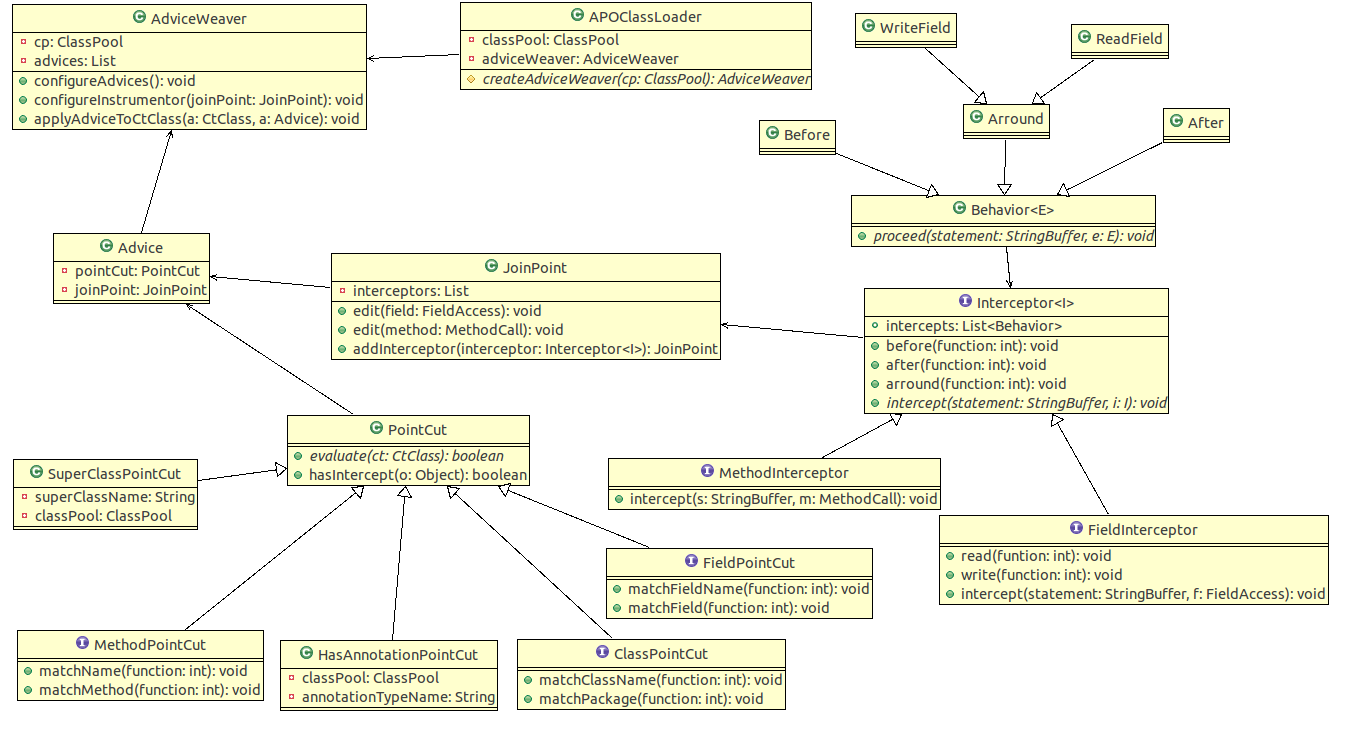
\includegraphics[width=450px, height=377px]{img/apo}
		\caption{Diagrama UML de la herramienta APO}
		\label{aopImage}
	\end{figure}	 
	
	
	\begin{figure}[h]
		\begin{lstlisting}
$Object oldValue = $oldValue;
$originalAsigment;
$this.firePropertyChange('$fieldName', oldValue, $newValue);
		\end{lstlisting}
		\caption{Fragmento de código del framework POO}
		\label{pooCode}
	\end{figure}
	
	
	\begin{table*}[h]\centering
		\ra{1.3}
		\begin{tabular}{|+l^l^p{7cm}|}\toprule			
			\hline
			\rowstyle{\bfseries}%
				Expr. APO & Expr. Javassist & Significado \\
			\hline
				\$Object & java.lang.Object & El nombre completo de la clase Object \\
			\hline
				\$this & \$0 & El objeto receptor del mensaje.\\
			\hline
				\$newValue & \$1 & El primer parámetro del método. \\
			\hline
				\$oldValue &  \$0.getAtribute() & El valor del atributo antes de
			la asignación que está siendo modificada.\\
			\hline
				\$originalAsigment & \$0.atribute = \$1 & La asignación del atributo con el
			primer parámetro del método.\\
			\hline
				``\$fieldName'' & ``atribute'' & El nombre del atributo como un String.\\
			\hline
		\bottomrule
		\end{tabular} 
		\caption{Tabla de equivalencia de expresiones. ``atribute'' es el nombre del atributo propiamente dicho.}
		\label{table}
	\end{table*}
	
	APO es una herramienta abstracta, es decir, por sí sola no define ninguna modificación sobre las clases.
	En cambio, hay que configurarlo adecuadamente para obtener el resultado deseado. 
	POO y POT se contruyeron siguiendo esta filosofía de creación de aspectos.
